\PassOptionsToPackage{unicode}{hyperref}
\documentclass[aspectratio=1610, 9pt]{beamer}

\usetheme{vertex}
\setbeamersize{text margin left=5mm,text margin right=5mm} 

\newfontfamily\zigarette{TeX Gyre Heros}

\usepackage[main=ngerman, english]{babel}

\usepackage[autostyle]{csquotes}
\renewcommand{\mkblockquote}[4]{foo#1#2\par\hfill\footnotesize#4#3}

\usepackage[firstinits=true, style=authortitle]{biblatex}
\addbibresource{references.bib}
\DefineBibliographyStrings{german}{andothers = {{et\,al\adddot}}}  % replace u.a. with et al.

\usepackage{tcolorbox}

\usepackage{siunitx}

\usepackage{grffile}
\usepackage{graphicx}
\usepackage{tikz}
\usetikzlibrary{calc}
\usetikzlibrary{positioning}
\tikzset{
  invisible/.style={opacity=0,text opacity=0},
  visible on/.style={alt={#1{}{invisible}}},
  alt/.code args={<#1>#2#3}{%
    \alt<#1>{\pgfkeysalso{#2}}{\pgfkeysalso{#3}} % \pgfkeysalso doesn't change the path
  },
}

\usepackage{hyperref}
\usepackage{bookmark}


\title{Farbwahrnehmung und Datenvisualisierung}
\author[maxnoe]{Maximilian Nöthe}
\date[SoAk19]{PeP et al. Sommerakademie 2019}
\institute{PeP et Al.}

\begin{document}
\maketitle

\begin{frame}[t]{Überblick}
  \begin{tikzpicture}[remember picture, overlay, shift=(current page.center)]
    \tikzset{arrow/.style={->, line width=3pt, color=gray}}
    \node[anchor=center, fill=black, text=green!70!white] (DATA) at (-5, -3.5) {\tiny%
      \begin{tabular}{@{}r@{ }r@{ }r@{ }r@{ }r@{}}
        129 & 135 & 184 & 211 & 167 \\
        126 & 122 & 167 & 217 & 194 \\
        121 & 97  & 110 & 195 & 212 \\
        112 & 93  & 60  & 108 & 158 \\
        96  & 59  & 43  & 51  & 51  \\
      \end{tabular}
    };
    \node[anchor=center] (RGB) at (-5, -2) {\texttt{\#ff0033}};
    \node[anchor=center] (MON) at (-5, 0) {%
      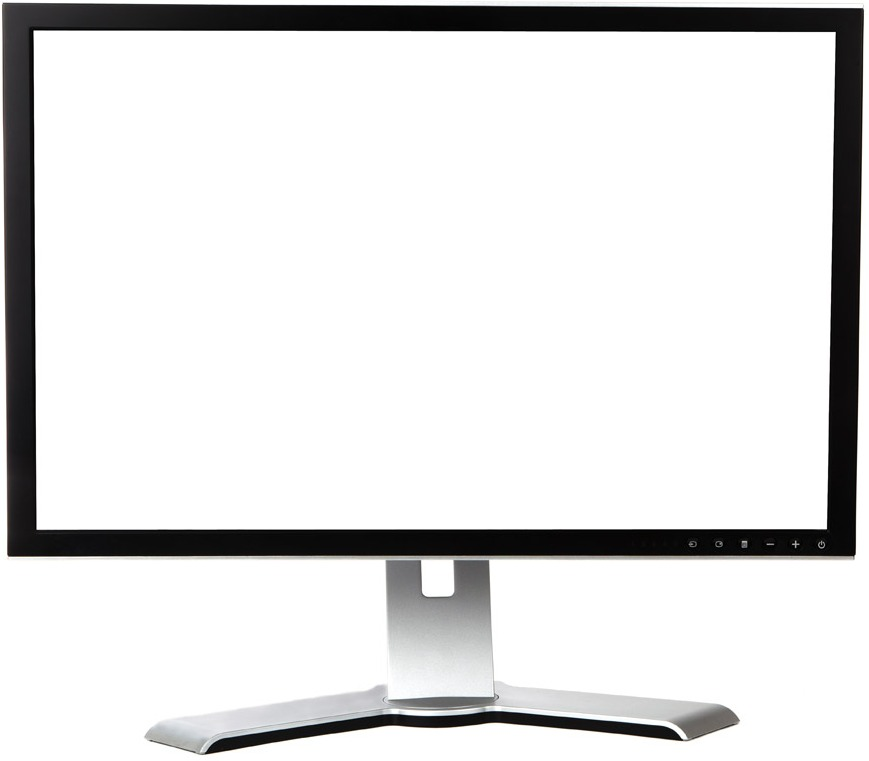
\includegraphics[height=1.5cm]{images/monitor.jpg}%
    };

    \node[anchor=center] (LIGHT) at (-3, 2) {%
      \begin{tikzpicture}[scale=0.25]
        \draw [draw=none, fill=red] (90:1.5) circle (2cm);
\draw [draw=none, fill=green] (-30:1.5) circle (2cm);
\draw [draw=none, fill=blue] (210:1.5) circle (2cm);

% Draw areas where two of the three primary colors are overlapping.
% These areas are the secondary colors yellow, cyan and magenta.
\begin{scope} % red + green = yellow
	\clip (90:1.5) circle(2cm);
	\draw [draw=none, fill=yellow] (-30:1.5) circle (2cm);
\end{scope} % blue + red = magenta
\begin{scope}
	\clip (210:1.5) circle(2cm);
	\draw [draw=none, fill=magenta] (90:1.5) circle (2cm);
\end{scope}
\begin{scope} % green + blue = cyan
	\clip (-30:1.5) circle(2cm);
	\draw [draw=none, fill=cyan] (210:1.5) circle (2cm);
\end{scope}

% Draw the center area which consists of all the primary colors.
\begin{scope} % red + green + blue = white
	\clip (90:1.5) circle(2cm);
	\clip (210:1.5) circle(2cm);
	\draw [draw=none, fill=white] (-30:1.5) circle (2cm);	
\end{scope}

      \end{tikzpicture}
    };

    \node[anchor=center, text width = 2.5cm] (EYE) at (1, 2) {{%
      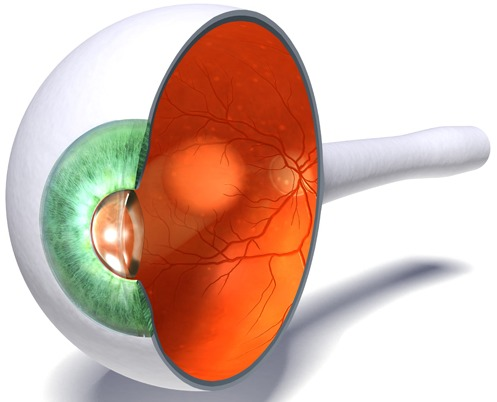
\includegraphics[width=\linewidth]{images/eye.jpg}\tiny\\[-2ex]
      [www.medicalgracphics.com]
    }};

    \node[anchor=center, text width = 3.5cm] (BRAIN) at (5, -1) {{%
      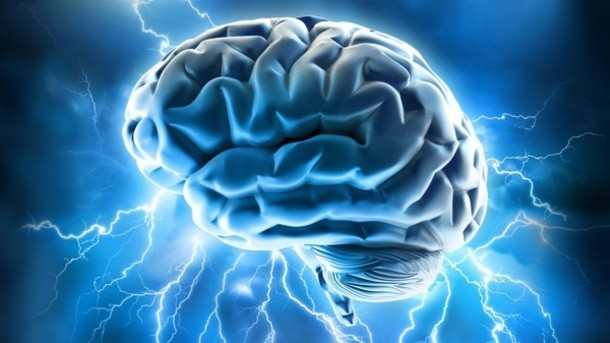
\includegraphics[width=\linewidth]{images/brain.jpg}%
    }};

    \node[left=0.2cm of DATA]  {\Large\bfseries Daten};
    \node[left=0.2cm of RGB]  {\Large\bfseries RGB};
    \node[left=0.2cm of MON]  {\Large\bfseries Monitor};
    \node[above=0.0cm of LIGHT]  {\Large\bfseries Licht};
    \node[above=0.0cm of EYE]  {\Large\bfseries Auge/Retina};
    \node[left=0.2cm of BRAIN]  {\Large\bfseries Gehirn};
    \node[below=0.0cm of BRAIN]  {\Large\bfseries Subjektive Wahrnehmung};

    \draw[arrow] (DATA.north) -- (RGB.south);
    \draw[arrow] (RGB.north) -- (MON.south);
    \draw[arrow] (MON.north) to[out=90, in=180] (LIGHT.west);
    \draw[arrow] (LIGHT.east) -- (EYE.west);
    \draw[arrow] (EYE.east) to[out=0, in=90] (BRAIN.north);
  \end{tikzpicture}
\end{frame}

\section{Menschliche Farbwahrnehmung}
\bumper{Menschliche Farbwahrnehmung}

\begin{frame}[c]{Geschichte}
  \begin{columns}[onlytextwidth]
    \hfill
    \begin{column}{0.59\textwidth}
      \begin{itemize}
        \item Erste physiologische Versuche durch Johann Wolfgang von Goethe (Zur Farbenlehre, 1810) \\
        \item Dreifarbentheorie (Young \& v. Helmholtz, 1804 / 1850)
        \item Gegenfarbtheorie (Hering 1878) \\
          \begin{tabular}{r @{${}⟷  {}$} l}
            blau & gelb \\
            rot & grün \\
            hell & dunkel \\
          \end{tabular}
        \item Erster Nachweis der Zapfen (Svaetichin, 1956) 
      \end{itemize}
    \end{column}
    \hfill%
    \begin{column}{0.39\textwidth}
      \hfill%
      \vfill%
      \centering
      \only<1>{%
        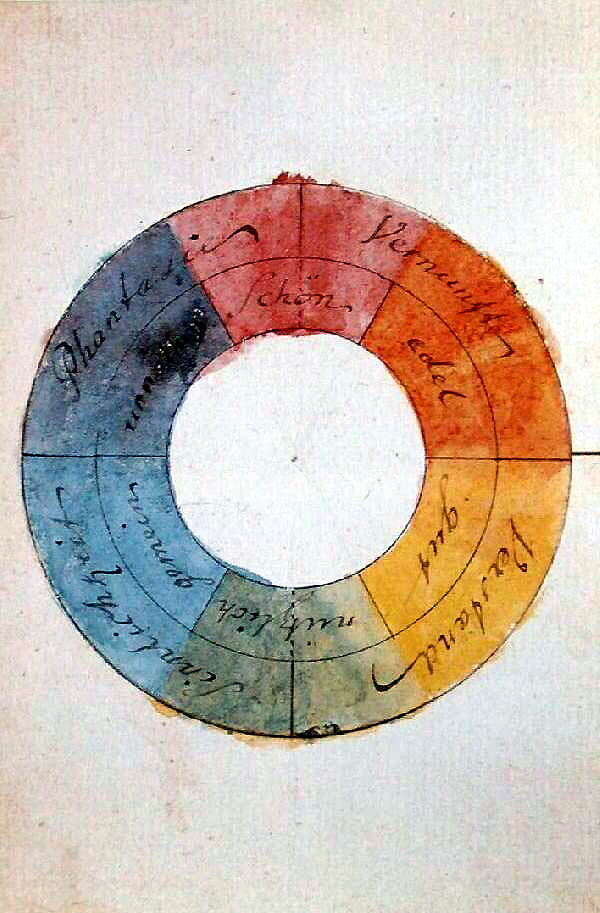
\includegraphics[width=\linewidth, height=0.90\textheight, keepaspectratio]{images/goethe_farbenkreis.jpg}

        [Goethe, 1809]
      }%
      \only<2>{%
        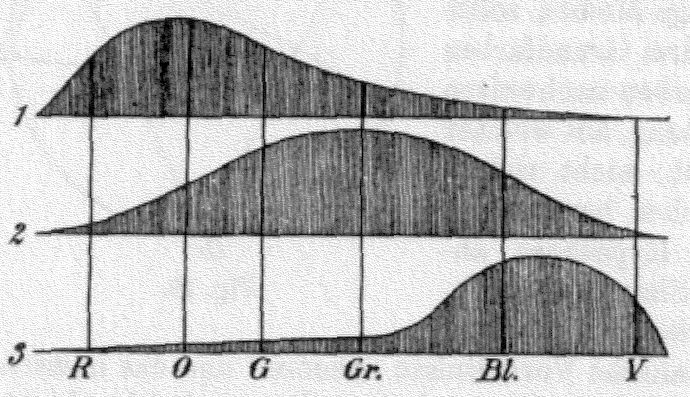
\includegraphics[width=\linewidth]{images/YoungHelm.jpg}

        [v. Helmholtz, 1894]
      }%
      \vfill%
    \end{column}%
  \end{columns}%
\end{frame}

\begin{frame}[c, plain]
  \centering
  \begin{tikzpicture}[shift=(current page.center), remember picture, overlay]
    \fill[color=green] (0, 0) rectangle (-0.2\textwidth, 0.2\textwidth);
    \fill[color=yellow] (0, 0) rectangle (0.2\textwidth, 0.2\textwidth);
    \fill[color=blue] (0, 0) rectangle (-0.2\textwidth, -0.2\textwidth);
    \fill[color=red] (0, 0) rectangle (0.2\textwidth, -0.2\textwidth);
    \fill[color=black] (0, 0) circle (0.01\textwidth);
  \end{tikzpicture}
\end{frame}

\begin{frame}[c, plain]
  \begin{tikzpicture}[remember picture, overlay, shift=(current page.center)]
    \fill[color=black] (0, 0) circle (0.01\textwidth);
  \end{tikzpicture}
\end{frame}


\begin{frame}[t]{Zapfen – Farben}
  \includegraphics{build/plots/cone_response.pdf} 
\end{frame}

\begin{frame}[t]{Zapfen – Helligkeit}
  \includegraphics{build/plots/photopic.pdf} 
\end{frame}


\begin{frame}{Lichtspektren - Metamerismus}

  \begin{columns}[onlytextwidth]
    \begin{column}{0.35\textwidth}
      \centering%
      \includegraphics[width=\linewidth]{build/plots/spectrum0.pdf}\\[0.2cm]
      oder\\
      \includegraphics[width=\linewidth]{build/plots/spectrum1.pdf}\\[0.2cm]
      oder\\
      \includegraphics[width=\linewidth]{build/plots/spectrum2.pdf}\\[0.2cm]
      \Huge $1\times N$
    \end{column}
    \begin{column}{0.04\textwidth}
      \begin{tikzpicture}
        \fill[black] (0, 0) circle (0.3cm);
      \end{tikzpicture}
    \end{column}
    \begin{column}{0.35\textwidth}
      \centering%
      \includegraphics[width=\textwidth]{build/plots/cone_response_matrix.pdf}
      \Huge $N \times 3$
    \end{column}
    \begin{column}{0.20\textwidth}
      \Huge ${}=3$ Reize
    \end{column}
  \end{columns}
  \vspace{0.5cm}
  Viele verschiedene Spektren können die gleichen Farbreize erzeugen \\
  Lineare Algebra!
\end{frame}


\section{Farbtheorie}
\bumper{Farbtheorie}

\begin{frame}{Farbräume}
  \begin{itemize}
    \item Farben lassen sich als 3-Vektoren Darstellen
    \item Geeignete Basis?
    \item Welche Bedeutung haben Abstände?
    \item Wie finden wir Größen wie Buntton, Sättingung, Helligkeit wieder?
  \end{itemize}

  \Large $⇒{}$ Entwicklung zahlreicher Farbmodelle
\end{frame}%

\begin{frame}{CIE 1931}
  \begin{columns}[onlytextwidth]%
    \begin{column}{0.495\textwidth}%
      \includegraphics{build/plots/gamut.pdf}
    \end{column}%
    \begin{column}{0.495\textwidth}%
      \begin{itemize}
        \item \enquote{Standard-Beobachter} über Messungen der Zapfenantwort
        \item Alle wahrnehmbaren Farben
        \item Lineare Tristimulus-Basis XYZ
        \item Referenz für fast alle anderen Farbräume
        \item Aber: Abstände bilden nicht den wahrgenommen Unterschied dar
      \end{itemize}
    \end{column}%
  \end{columns}%
\end{frame}

\begin{frame}{CIE L*a*b 1976}
\end{frame}

\begin{frame}{RGB – Monitore, Beamer, etc.}
      \includegraphics{build/plots/gamut_srgb.pdf}
\end{frame}

\begin{frame}{CMYK – Warum Drucken schwer ist}
\end{frame}


\section{Farbfehlsichtigkeit}
\bumper{Farbfehlsichtigkeit}
\begin{frame}[t]{Farbfehlsichtigkeit}
  \begin{center}
    \includegraphics{build/plots/colorblind_response.pdf}
  \end{center}
  
  Prozentzahlen für weiße Männer. \\
  Wird X-chromosonal vererbt ${}⇒{}$ Frauen ca. quadratisch weniger\\
  Andere Farbfehlsichtigkeiten ${}< \SI{0.01}{\percent}$
\end{frame}

\begin{frame}[t]{Farbfehlsichtigkeit}
  \begin{columns}[onlytextwidth]%
    \begin{column}{0.495\textwidth}%
      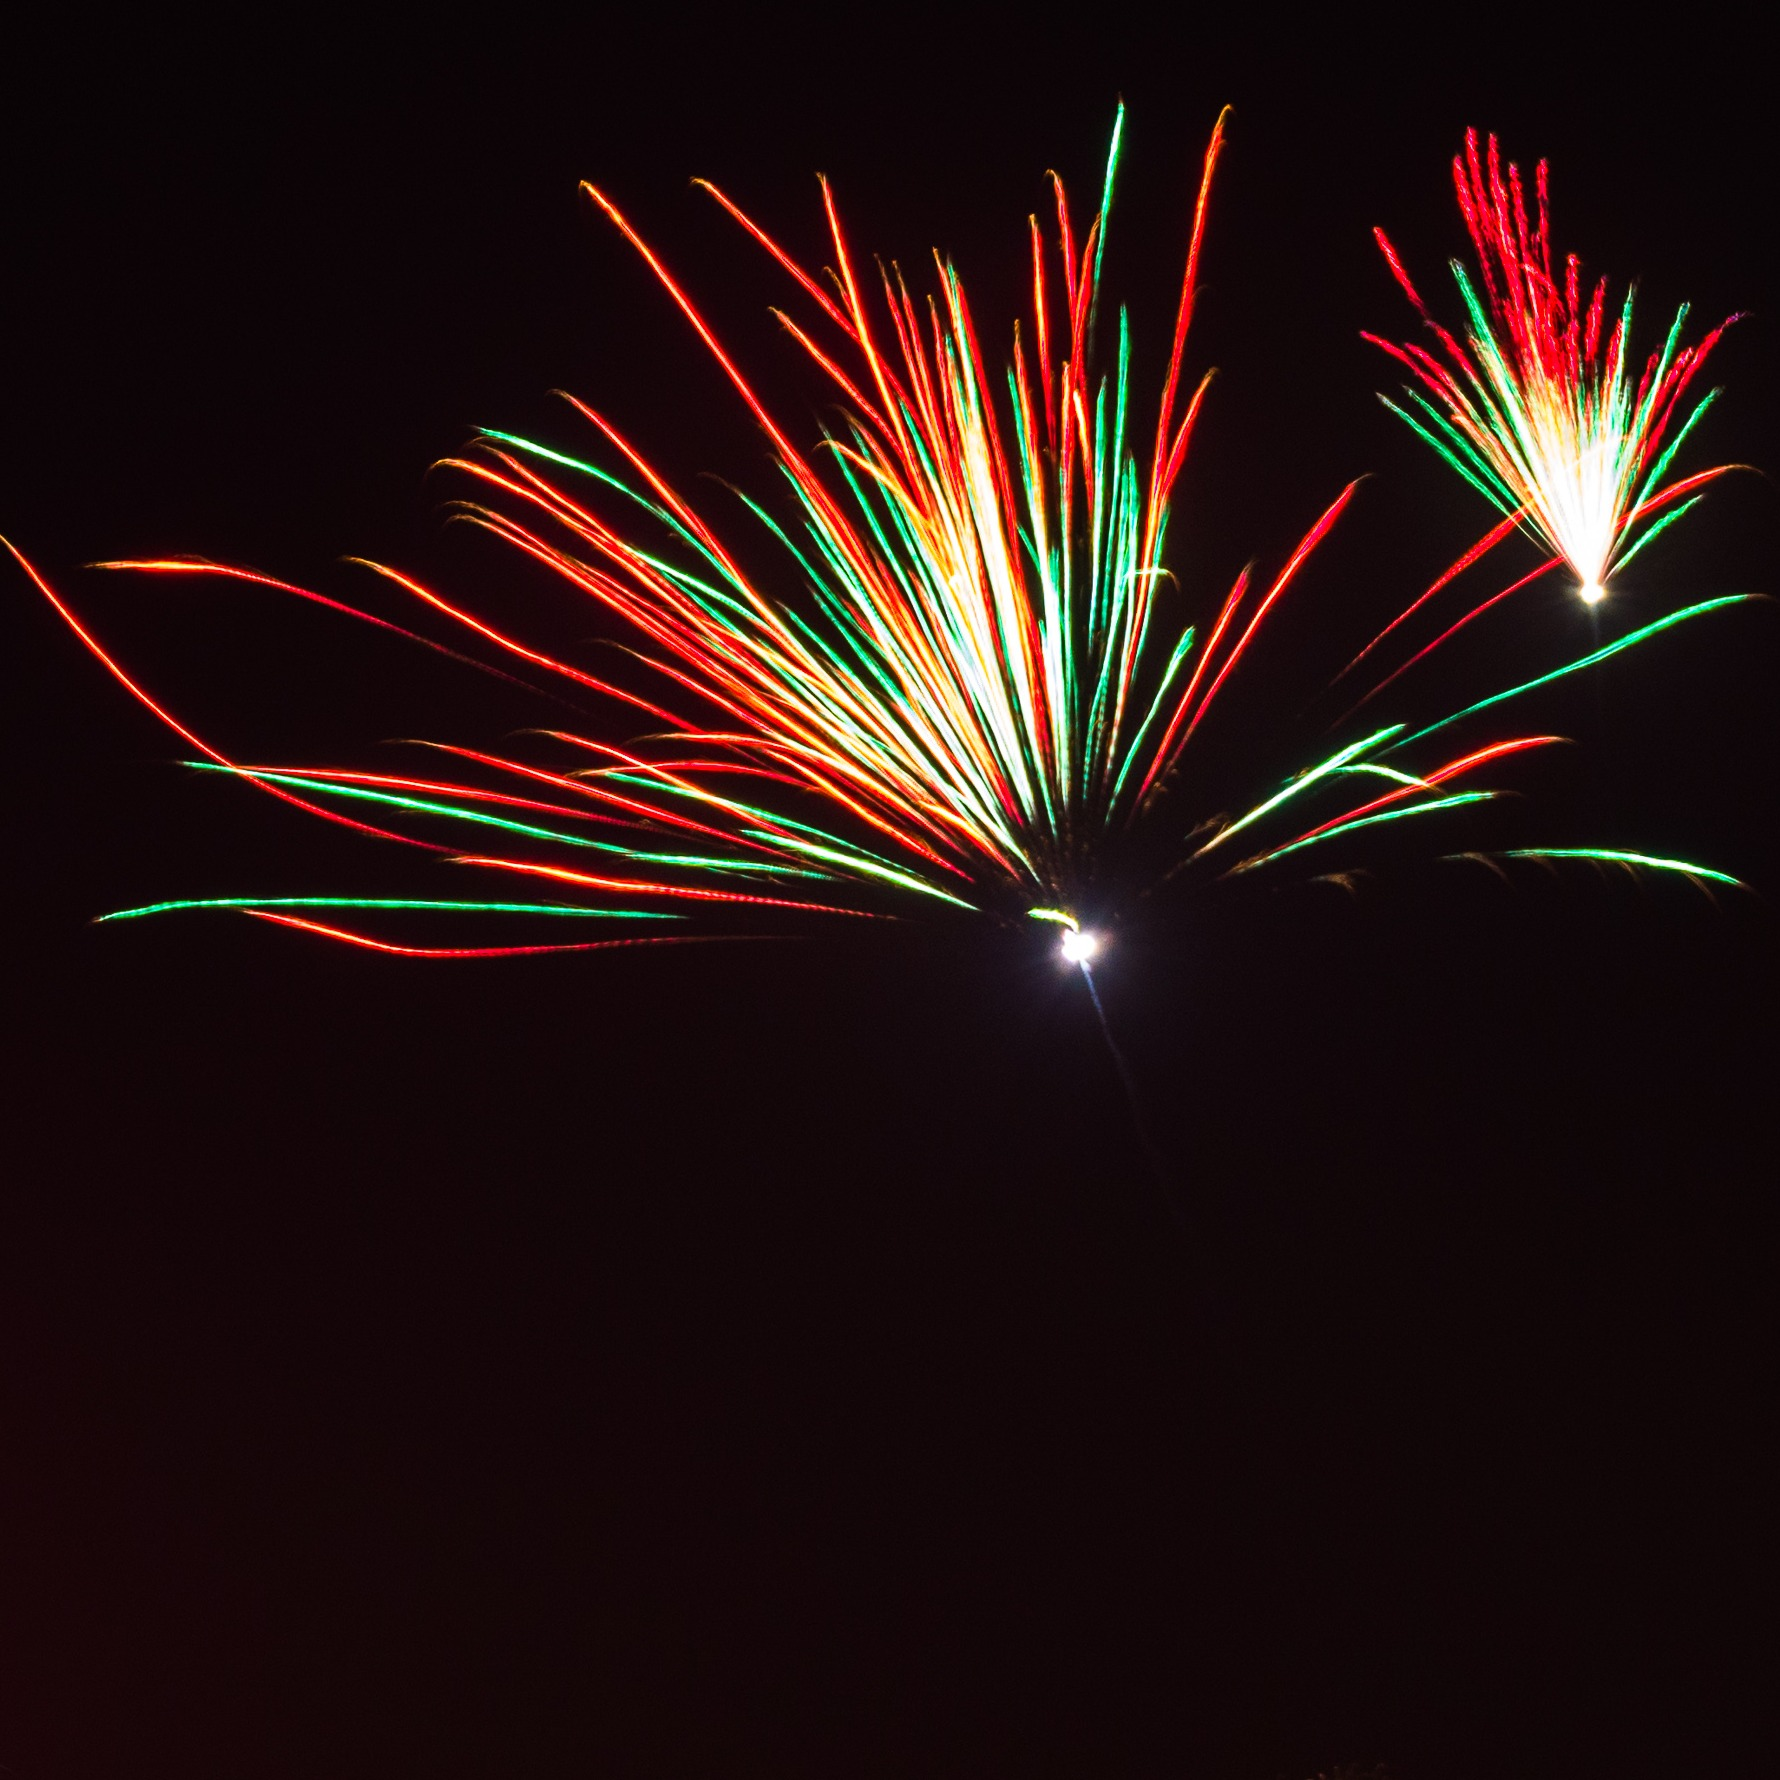
\includegraphics[width=\linewidth]{images/feuerwerk.jpg}\\
    \end{column}%
    \hfill%
    \begin{column}{0.495\textwidth}%
      \only<1>{\includegraphics[width=\linewidth]{build/plots/fireworks_deuter_50.jpg}}%
      \only<2>{\includegraphics[width=\linewidth]{build/plots/fireworks_deuter_100.jpg}}%
    \end{column}%
  \end{columns}%

  \begin{center}%
    \only<1>{Moderate Deuteranomalie}%
    \only<2>{Deuteranopie}%
  \end{center}%
\end{frame}




\section{Datenvisualisierung}
\bumper{Datenvisualisierung}

\begin{frame}[t]{Warum?}
  \begin{tikzpicture}[remember picture, overlay, shift=(current page.center)]
    \node[anchor=north west, fill=black, text=green!70!white] (A) at (-0.5\textwidth, 0.4\textheight) {
      \tiny\input{build/img.tex}%
    };
    \node [xshift=1cm, yshift=-1.7cm, visible on=<2->] at (A.south) {%
      \includegraphics{build/plots/u_cmap.pdf}%
    }; 
    \node[anchor=south east, visible on=<3->] (B) at (0.5\textwidth, -0.5\textheight) {{
      \includegraphics[height=4cm]{build/plots/u_sw.png}
    }};
    \draw[line width=5pt, ->, visible on=<2->] (A.south) to [out=270, in=180] (B.west);
  \end{tikzpicture}%
\end{frame}

\begin{frame}[t]{Verschiedene Colormaps}
  \begin{columns}[onlytextwidth]%
    \begin{column}{0.52\textwidth}%
      \includegraphics{build/plots/u_cmaps.pdf}
    \end{column}%
    \hfill%
    \begin{column}{0.47\textwidth}%
      \begin{itemize}
        \item Was macht eine gute Colormap aus?
        \item Welche verschiedenen Sorten gibt es?
        \item Was für welche Daten?
        \item Normierung?
      \end{itemize}
    \end{column}%
  \end{columns}%
\end{frame}

\begin{frame}{Kriterien für eine gute Colormap}
  \begin{itemize}
    \item Bunt
    \item Sieht gut aus\\[2\baselineskip]
    \item Exakte Repräsententation der Daten (\enquote{Gleichmäßige Wahrnehmung})
    \item Auch in schwarz-weiß 
    \item Auch für Menschen mit Farbfehlsichtigkeit
  \end{itemize}
\end{frame}

\begin{frame}[plain]{jet}
  \makebox[\linewidth]{\includegraphics[width=\paperwidth, height=\paperheight, keepaspectratio]{build/plots/cmap_jet.pdf}}
\end{frame}

\begin{frame}[plain]{viridis}
  \makebox[\linewidth]{\includegraphics[width=\paperwidth, height=\paperheight, keepaspectratio]{build/plots/cmap_viridis.pdf}}
\end{frame}


\begin{frame}{Spezielle Colormaps für spezielle Daten}%
  \only<1>{\includegraphics{build/plots/europe_jet.pdf}}%
  \only<2>{\includegraphics{build/plots/europe_divnorm.pdf}}%
\end{frame}%


\begin{frame}[t]{Wahl der Farbskala hat Konsequenzen}
  \begin{center}
    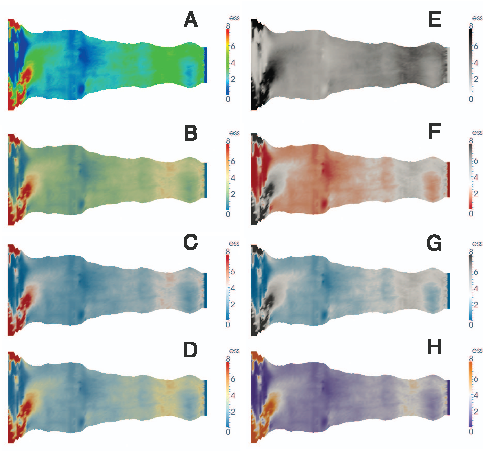
\includegraphics[height=0.7\textheight]{images/heartdisease.pdf}
  \end{center}

  \leavevmode
  \foreignblockquote{english}{%
    We show statistically significant results demonstrating [...]
    that a perceptually appropriate color map
    leads to \textbf{fewer diagnostic mistakes} than a rainbow color map.%
  }\\[0.5\baselineskip]
  \small\cite{heartdisease}
\end{frame}


\begin{frame}[t]{Wahl der Farbskala hat Konsequenzen}  
  \centering

  \includegraphics[height=0.7\textheight]{build/plots/norainbow.pdf}

  \begin{tcolorbox}[colframe=black, colback=white, fontupper=\raggedright\bfseries\zigarette, width=0.68\textwidth, boxrule=4pt, sharp corners]
    Benutzung der Rainbow-Colormap fügt Ihnen
    und den Menschen in Ihrer Umgebung erheblichen Schaden zu.
  \end{tcolorbox}
\end{frame}


\end{document}
